%-------------------------------------------------------------------------------
%                      PREAMBLE - Document Declaration
%-------------------------------------------------------------------------------
\documentclass[a4paper, leqno, 12pt]{article}

\usepackage{setspace}
\usepackage[asymmetric]{geometry}
\usepackage{amsmath}
\usepackage{graphicx}
\usepackage{graphics}
\usepackage{calc}
\usepackage{xintexpr}
% \usepackage{l3regex}
\usepackage{expl3}
\usepackage{pgfplots}
\usepackage{amsmath}
\usepackage{multicol}
\pgfplotsset{compat=1.16}


\geometry{hmargin=2.3cm,
vmargin=2.5cm }

\newenvironment{top_enumerate}{
\begin{enumerate}
  \setlength{\itemsep}{2em}
  \setlength{\topsep}{-0pt}
  \setlength{\partopsep}{-0pt}
}{\end{enumerate}}

\newlength{\EqL}
\newlength{\RunL}
\setlength{\RunL}{0pt}
\newcommand{\EqContent}{foo}
\renewcommand{\theequation}{\alph{equation}}

\ExplSyntaxOn
\tl_new:N \l_mathexp_tl
\cs_new:Npn \nodollar #1 {
    \tl_set:Nn \l_mathexp_tl {#1}
    \regex_replace_all:nnN { \$ } {} \l_mathexp_tl
    \tl_use:N \l_mathexp_tl
}
\ExplSyntaxOff

%-------------------------------------------------------------------------------
%                               DOCUMENT
%-------------------------------------------------------------------------------
\begin{document}
\singlespacing
\begin{center}
\textbf{
ECON101 - Maths seminar material - Week 1\\
\bigskip
Algebra
}
\end{center}
\bigskip

\begin{top_enumerate}

\item Given the following pair of coordinate points $(x,y)$, find and sketch the linear equation $y = ax + b$. Where necessary, make sure you enter any rational number as a fraction, and not as a decimal number.
 
\setcounter{equation}{0}  % reset counter 
\begin{enumerate}
	\setlength{\topsep}{-0pt}
	\setlength{\partopsep}{-0pt}
	\setlength{\itemsep}{10pt}
			\item $A= ({-2},{-1}),\, B= ({9},{-4})$
	 \quad \textbf{[3]}
\end{enumerate}\addtocounter{enumi}{-1}
\item Solution:
 
\setcounter{equation}{0}  % reset counter 
\begin{enumerate}
	\setlength{\topsep}{-0pt}
	\setlength{\partopsep}{-0pt}
	\setlength{\itemsep}{10pt}
			\item First, the slope is linear, which means that $a = \frac{y_B-y_A}{x_B-x_A}$. Once $a$ is known, its value can be replaced in the linear expression $y = ax + b$, and the $x$/$y$ values of either point can be used to determine the value of $b$.
	
	For $A= ({-2},{-1}),\, B= ({9},{-4})$:
	\[
	\left\{\begin{aligned}
	a & = \frac{y_B-y_A}{x_B-x_A} = \frac{{-4}-{-1}}{{9}-{-2}} = \frac{{-3}}{{11}}\\
	b & = y_A -ax_A = {-1} - \frac{{-3}}{{11}}{-2} = \frac{{-17}}{{11}} \\
	 \end{aligned}\right.
	\]
	
	Therefore $y = \frac{{-17}}{{11}} + \frac{{-3}}{{11}}x \approx {-1.545} { } {-0.273}x$
	
	\begin{center}
	\begin{tikzpicture}
	\begin{axis}[
	xlabel=$x$,
	ylabel=$y$,
	axis lines = center,
	legend style={at={(0.5,-0.1)},anchor=north,draw=none,legend columns=-1}]
	\addplot[domain=-10:10,color=blue,]{ -17/11 +-3/11*x};
	\addlegendentry{$y=ax+b$}
	\addplot[mark=*]coordinates {(-2,-1)};
	\addlegendentry{$A$}
	\addplot[mark=o]coordinates {(9,-4)};
	\addlegendentry{$B$}
	\end{axis}
	\end{tikzpicture}
	\end{center}
	 \quad \textbf{}
\end{enumerate}\newpage
\item Given \(A=\left( {\begin{array}{cc}
   {9} & {8} \\
   {2} & {-5} \\
 \end{array} } \right) \), \(B=\left( {\begin{array}{cc}
     {-1} & {2} \\
     {1} & {1} \\
    \end{array} } \right) \), calculate the following matrix operations. Where necessary, make sure you keep any rational number as a fraction, and not as a decimal number.
 \\ 
\setcounter{equation}{0}  % reset counter 
\setlength{\RunL}{0pt}
	\renewcommand{\EqContent}{\nodollar{$A+B$
	\qquad\textbf{[1]}}}
	\settowidth{\EqL}{$\qquad\EqContent\qquad$}
	\setlength{\RunL}{\RunL+\EqL}
	\xintifboolexpr { \RunL > 0.667*\textwidth }
		{\setlength{\RunL}{0pt}
		\\}
		{}
	\begin{minipage}{\EqL}
	\begin{equation}
	\EqContent
	\end{equation}
	\end{minipage}
	\renewcommand{\EqContent}{\nodollar{${2}A-{3}B$
	\qquad\textbf{[1]}}}
	\settowidth{\EqL}{$\qquad\EqContent\qquad$}
	\setlength{\RunL}{\RunL+\EqL}
	\xintifboolexpr { \RunL > 0.667*\textwidth }
		{\setlength{\RunL}{0pt}
		\\}
		{}
	\begin{minipage}{\EqL}
	\begin{equation}
	\EqContent
	\end{equation}
	\end{minipage}
	\renewcommand{\EqContent}{\nodollar{${5}A+{2}B$
	\qquad\textbf{[1]}}}
	\settowidth{\EqL}{$\qquad\EqContent\qquad$}
	\setlength{\RunL}{\RunL+\EqL}
	\xintifboolexpr { \RunL > 0.667*\textwidth }
		{\setlength{\RunL}{0pt}
		\\}
		{}
	\begin{minipage}{\EqL}
	\begin{equation}
	\EqContent
	\end{equation}
	\end{minipage}
	\renewcommand{\EqContent}{\nodollar{$AB$
	\qquad\textbf{[3]}}}
	\settowidth{\EqL}{$\qquad\EqContent\qquad$}
	\setlength{\RunL}{\RunL+\EqL}
	\xintifboolexpr { \RunL > 0.667*\textwidth }
		{\setlength{\RunL}{0pt}
		\\}
		{}
	\begin{minipage}{\EqL}
	\begin{equation}
	\EqContent
	\end{equation}
	\end{minipage}
	\renewcommand{\EqContent}{\nodollar{$|A|$
	\qquad\textbf{[2]}}}
	\settowidth{\EqL}{$\qquad\EqContent\qquad$}
	\setlength{\RunL}{\RunL+\EqL}
	\xintifboolexpr { \RunL > 0.667*\textwidth }
		{\setlength{\RunL}{0pt}
		\\}
		{}
	\begin{minipage}{\EqL}
	\begin{equation}
	\EqContent
	\end{equation}
	\end{minipage}
	\renewcommand{\EqContent}{\nodollar{$|B|$
	\qquad\textbf{[2]}}}
	\settowidth{\EqL}{$\qquad\EqContent\qquad$}
	\setlength{\RunL}{\RunL+\EqL}
	\xintifboolexpr { \RunL > 0.667*\textwidth }
		{\setlength{\RunL}{0pt}
		\\}
		{}
	\begin{minipage}{\EqL}
	\begin{equation}
	\EqContent
	\end{equation}
	\end{minipage}
	\renewcommand{\EqContent}{\nodollar{$A^{-1}$
	\qquad\textbf{[2]}}}
	\settowidth{\EqL}{$\qquad\EqContent\qquad$}
	\setlength{\RunL}{\RunL+\EqL}
	\xintifboolexpr { \RunL > 0.667*\textwidth }
		{\setlength{\RunL}{0pt}
		\\}
		{}
	\begin{minipage}{\EqL}
	\begin{equation}
	\EqContent
	\end{equation}
	\end{minipage}
	\renewcommand{\EqContent}{\nodollar{$B^{-1}$
	\qquad\textbf{[2]}}}
	\settowidth{\EqL}{$\qquad\EqContent\qquad$}
	\setlength{\RunL}{\RunL+\EqL}
	\xintifboolexpr { \RunL > 0.667*\textwidth }
		{\setlength{\RunL}{0pt}
		\\}
		{}
	\begin{minipage}{\EqL}
	\begin{equation}
	\EqContent
	\end{equation}
	\end{minipage}
\addtocounter{enumi}{-1}
\item Solutions:
 
\setcounter{equation}{0}  % reset counter 
\begin{enumerate}
	\setlength{\topsep}{-0pt}
	\setlength{\partopsep}{-0pt}
	\setlength{\itemsep}{10pt}
			\item $A+B = \left( {\begin{array}{cc}
	    {8} & {10} \\
	    {3} & {-4} \\
	 \end{array} } \right) $
	 \quad \textbf{}
		\item ${2}A-{3}B = \left( {\begin{array}{cc}
	   {21} & {10} \\
	   {1} & {-13} \\
	 \end{array} } \right) $
	 \quad \textbf{}
		\item ${5}A+{2}B = \left( {\begin{array}{cc}
	   {43} & {44} \\
	   {12} & {-23} \\
	 \end{array} } \right) $
	 \quad \textbf{}
		\item $AB = \left( {\begin{array}{cc}
	   {-1} & {26} \\
	   {-7} & {-1} \\
	 \end{array} } \right) $
	 \quad \textbf{}
		\item $|A| = {9} \times {-5} - ({8} \times {2}) = {-61}$
	 \quad \textbf{}
		\item $|B| = {-1} \times {1} - ({2} \times {1}) = {-3}$
	 \quad \textbf{}
		\item $A^{-1} = \frac{\textrm{Adj}A}{|A|} = \left( {\begin{array}{cc}
	    \frac{{-5}}{{-61}} & \frac{{-8}}{{-61}} \\
	    \frac{{-2}}{{-61}} & \frac{{9}}{{-61}} \\
	  \end{array} } \right) \approx \left( {\begin{array}{cc}
	       {0.08} & {0.13} \\
	       {0.03} & {-0.15} \\
	      \end{array} } \right) $
	 \quad \textbf{}
		\item $B^{-1} = \frac{\textrm{Adj}B}{|B|} = \left( {\begin{array}{cc}
	    \frac{{1}}{{-3}} & \frac{{-2}}{{-3}} \\
	    \frac{{-1}}{{-3}} & \frac{{-1}}{{-3}} \\
	  \end{array} } \right) \approx \left( {\begin{array}{cc}
	       {-0.33} & {0.67} \\
	       {0.33} & {0.33} \\
	      \end{array} } \right)$
	 \quad \textbf{}
\end{enumerate}\newpage
\item Find the values of $x$ which solve the following equations. Note that $x_1 < x_2$ and make sure to enter your answers in square brackets, e.g.$[-5,3]$.
 
\setcounter{equation}{0}  % reset counter 
\begin{multicols}{2}
\begin{enumerate}
	\setlength{\topsep}{-0pt}
	\setlength{\partopsep}{-0pt}
	\setlength{\itemsep}{10pt}
			\item $-{2}x^2 + {10}x + {9} = 0$
	 \quad \textbf{[3]}
		\item $x^2 + {20}x + {11} = 0$
	 \quad \textbf{[3]}
\end{enumerate}\end{multicols}\addtocounter{enumi}{-1}
\item Solutions:
 
\setcounter{equation}{0}  % reset counter 
\begin{enumerate}
	\setlength{\topsep}{-0pt}
	\setlength{\partopsep}{-0pt}
	\setlength{\itemsep}{10pt}
			\item The discriminant of the quadratic is:
	\[
	{10}^2+4\cdot{2}\cdot{9} = {100} + {72} = {172}
	\]
	As the discriminant is positive, there are two real roots to the quadratic:
	\[
	\left\{\begin{aligned}
	x_1 & = \frac{-{10}+\sqrt{{172}}}{-{4}} = \frac{{10}-\sqrt{{172}}}{{4}}\\
	x_2 & = \frac{-{10}-\sqrt{{172}}}{-{4}} = \frac{{10}+\sqrt{{172}}}{{4}}\\
	\end{aligned}\right.
	\]
	 \quad \textbf{}
		\item The discriminant of the quadratic is:
	\[
	{20}^2-4\cdot{11} = {400} - {44} = {356}
	\]
	As the discriminant is positive, there are two real roots to the quadratic:
	\[
	\left\{\begin{aligned}
	x_1 & = \frac{-{20}-\sqrt{{356}}}{2} = -{10} - \sqrt{{89}}\\
	x_2 & = \frac{-{20}+\sqrt{{356}}}{2} = -{10} + \sqrt{{89}}\\
	\end{aligned}\right.
	\]
	 \quad \textbf{}
\end{enumerate}\newpage
\item Solve the following pair of equations. Make sure to enter your answers in square brackets, e.g. $[5,-3]$.
 
\setcounter{equation}{0}  % reset counter 
\begin{enumerate}
	\setlength{\topsep}{-0pt}
	\setlength{\partopsep}{-0pt}
	\setlength{\itemsep}{10pt}
			\item $\left\{\begin{aligned}
	{16}x - {3}y & = {50}\\
	{8}x + {2}y & = {4}\\
	\end{aligned}\right.$
	 \quad \textbf{[2]}
\end{enumerate}\addtocounter{enumi}{-1}
\item The approach used here is to solve by adding/subtracting one equation from the other. Note that it can help to plot the two linear equations, the coordinates of the intersection point gives the solution to the system of equations.
 
\setcounter{equation}{0}  % reset counter 
\begin{enumerate}
	\setlength{\topsep}{-0pt}
	\setlength{\partopsep}{-0pt}
	\setlength{\itemsep}{10pt}
			\item Multiplying the second equation by ${2}$ and subtracting each side to the first equation:
	\[
	\begin{aligned}
	{16}x - {3}y - {2}({8}x + {2}y) & = {50} - {2}\cdot{4}\\
	{-7}y & = {42}\\
	y & = {-6}\\
	\end{aligned}
	\]
	Replace in equation 1 to solve for $x$
	\[
	\begin{aligned}
	{16}x-{3}\cdot{-6} & = {50}\\
	{16}x & = {32}\\
	x & = {2}\\
	\end{aligned}
	\]
	
	\begin{center}
	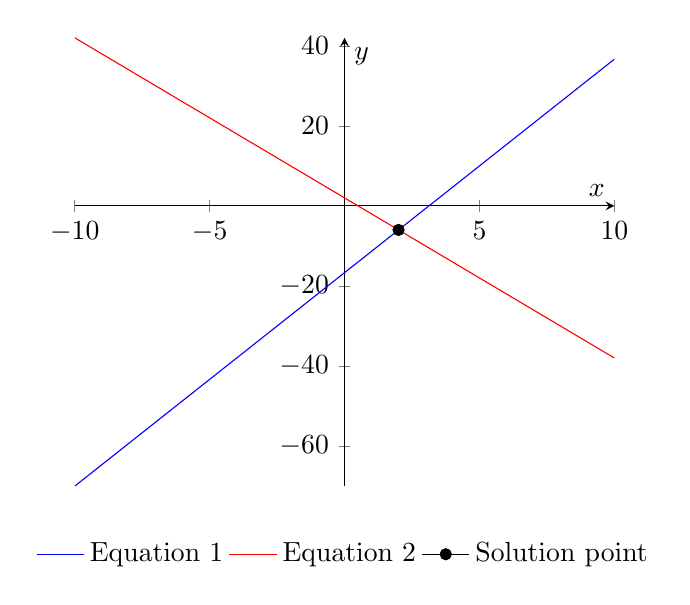
\begin{tikzpicture}
	\begin{axis}[
	xlabel=$x$,
	ylabel=$y$,
	axis lines = center,
	legend style={at={(0.5,-0.1)},anchor=north,draw=none,legend columns=-1}]
	\addplot[domain=-10:10,color=blue]{(16/3)*x-(50/3)};
	\addlegendentry{Equation 1}
	\addplot[domain=-10:10,color=red]{-(8/2)*x+(4/2)};
	\addlegendentry{Equation 2}
	\addplot[mark=*]coordinates {(2,-6)};
	\addlegendentry{Solution point}
	\end{axis}
	\end{tikzpicture}
	\end{center}
	 \quad \textbf{}
\end{enumerate}\newpage


\end{top_enumerate}
%-------------------------------------------------------------------------------
\end{document}
%-------------------------------------------------------------------------------
